\documentclass{article}
\usepackage[a4paper, total={5in, 8in}]{geometry}
\usepackage{amsmath}
\usepackage{amssymb}
\usepackage{amsthm}
\usepackage{xcolor}
\usepackage{graphicx}
\usepackage{hyperref}
\usepackage{listings}
\usepackage{float}
\usepackage{tikz}
\usepackage{multicol}
\usepackage{pgfplots}
\usepackage{subcaption}

\pgfplotsset{width=10cm,compat=1.9}

\colorlet{punct}{red!60!black}
\definecolor{background}{HTML}{EEEEEE}
\definecolor{delim}{RGB}{20,105,176}
\colorlet{numb}{magenta!60!black}

\lstdefinelanguage{json}{
    basicstyle=\normalfont\ttfamily,
    numbers=left,
    numberstyle=\scriptsize,
    stepnumber=1,
    numbersep=8pt,
    showstringspaces=false,
    breaklines=true,
    frame=lines,
    backgroundcolor=\color{background},
    literate=
     *{0}{{{\color{numb}0}}}{1}
      {1}{{{\color{numb}1}}}{1}
      {2}{{{\color{numb}2}}}{1}
      {3}{{{\color{numb}3}}}{1}
      {4}{{{\color{numb}4}}}{1}
      {5}{{{\color{numb}5}}}{1}
      {6}{{{\color{numb}6}}}{1}
      {7}{{{\color{numb}7}}}{1}
      {8}{{{\color{numb}8}}}{1}
      {9}{{{\color{numb}9}}}{1}
      {:}{{{\color{punct}{:}}}}{1}
      {,}{{{\color{punct}{,}}}}{1}
      {\{}{{{\color{delim}{\{}}}}{1}
      {\}}{{{\color{delim}{\}}}}}{1}
      {[}{{{\color{delim}{[}}}}{1}
      {]}{{{\color{delim}{]}}}}{1},
}

\lstdefinelanguage{xml}{
    basicstyle=\normalfont\ttfamily,
    numbers=left,
    numberstyle=\scriptsize,
    stepnumber=1,
    numbersep=8pt,
    showstringspaces=false,
    breaklines=true,
    frame=lines,
    backgroundcolor=\color{background},
    morestring=[b]",
    morestring=[s]{>}{<},
    morecomment=[s]{<?}{?>},
    morecomment=[s]{<!--}{-->},
    stringstyle=\color{blue},
    identifierstyle=\color{black},
    keywordstyle=\color{red},
    morekeywords={xmlns,version,type}
}
\lstdefinelanguage{proto}{
    basicstyle=\normalfont\ttfamily,
    numbers=left,
    numberstyle=\scriptsize,
    stepnumber=1,
    numbersep=8pt,
    showstringspaces=false,
    breaklines=true,
    frame=lines,
    backgroundcolor=\color{background},
    morestring=[b]",
    morestring=[s]{>}{<},
    morecomment=[s]{<?}{?>},
    morecomment=[s]{<!--}{-->},
    stringstyle=\color{blue},
    identifierstyle=\color{black},
    keywordstyle=\color{red},
    morekeywords={message, required, optional, repeated}
}

\author{Davi de Lima Cruz \\ Matrícula:474377}
\title{Relatório da Atvidade 01: Tamanho de envio de pacotes}
\date{\today}
\begin{document}
\maketitle
\section{Introdução}
Nessa atividade, foi pedido para avaliar o tamanho dos pacotes enviados por diferentes formas de envio de dados em Java.


\section{Metodologia}

\subsection{Dados}
Como pedido, avaliamos diferentes formam que o Java encia pacotes de dados. Sendo elas:
\begin{itemize}
    \item Serialização de objetos: nesse caso apenas implementamos a interface Serializable e enviamos o objeto.
    \item Serialização de objetos Customizando: para a Customizando implementamos a escrita e leitura do objeto de acordo com o seu tipo, em tese, isso poderia diminuir o tamanho do pacoete.
    \item Json: enviamos o arquivo em formato Json em formato de String.
    \item XML: enviamos o arquivo em formato XML em formato de String.
    \item Protobuf: usamos a classe gerada pelo protoc para enviar o arquivo.
\end{itemize}
Alem disso, escolhemos dois cenários para avaliar o tamanho do pacote, sendo eles:
\begin{enumerate}
    \item Lista de compras: contendo 5 itens onde cada item possui um nome, quantidade e unidade.
    \item Agenda de contatos: contendo 20 contatos onde cada contato possui um nome, telefone, email e foto.
\end{enumerate}
\newpage
Foi usada a mesma foto em todos os contatos e ela foi transformada em base64 para ser enviada.
\begin{figure}[H]
    \centering
    
\includegraphics[width=0.2\textwidth]{../client/src/main/java/data/foto.png}
    \caption{Foto usada nos contatos}
\end{figure}
O formato dos Json e XML fica no apendice para facilitar a leitura. Segue o protobuff usado para o caso da lista de compras e agenda de contatos.

\begin{lstlisting}[language=proto, caption=Protobuf utilizado na lista de compras.]
    syntax = "proto3";
    package data;
    option java_package = "data";
    
    message PCompras {
        repeated PItem lista_compras = 10;
    }
    message PItem {
        string nome = 1;
        float quantidade = 2;
        string unidade = 3;
    }
\end{lstlisting}

\begin{lstlisting}[language=proto, caption=Protobuf utilizado na agenda de contatos.]
    syntax = "proto3";
    package data;
    option java_package = "data";
    
    message PAgenda {
        repeated PContato contatos = 10;
    }
    message PContato {
        string nome = 1;
        string telefone = 2;
        string email = 3;
        string foto = 4;
    }
\end{lstlisting}

\subsection{Software}
Para fazer a medição dos pacotes foi criado um servidor e um cliente em Java.
O client mandava em sequencia um dado de cada tipo para cada caso em portas diferentes e
o servidor recebia sequencialmente.
Enquanto isso, o \textbf{tshark} capturava os pacotes e salvamos a porta e o tamanho do pacote em um arquivo.
A partir disso somamos o tamanho dos pacotes com o AWK.

\begin{table}[H]
    \centering
    \begin{tabular}{|c|c|c|}
        \hline
            & \multicolumn{2}{c|}{\textbf{Porta}} \\
            \hline
            \textbf{Tipo} & \textbf{Compras} & \textbf{Agenda} \\
            \hline
            Serialização & 5100 & 5200 \\
            Serialização Custom. & 5101 & 5201 \\
            Json & 5102 & 5202 \\
            XML & 5103 & 5203 \\
            Protobuf & 5104 & 5204 \\
            \hline
    \end{tabular}
    \caption{Portas utilizadas}
\end{table}


\section{Resultados}
\begin{figure}[H]
    \centering
    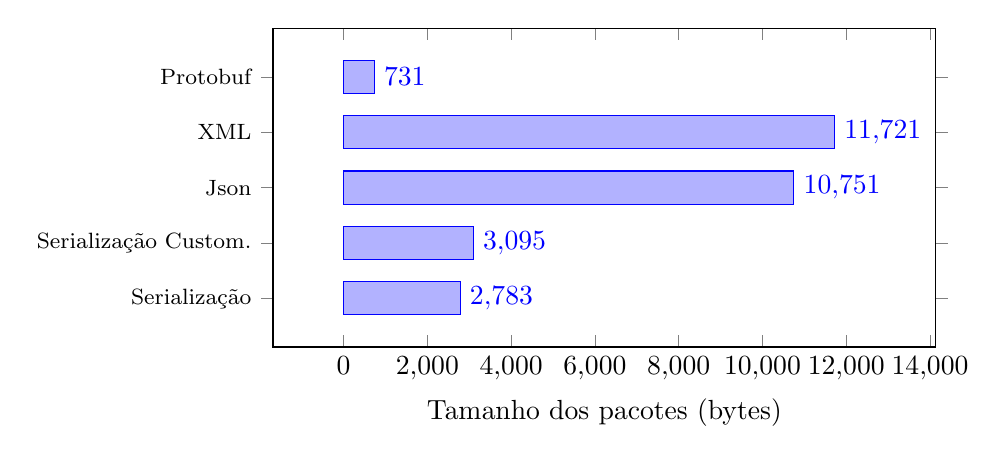
\begin{tikzpicture}
        \begin{axis}[
            symbolic y coords={ Serialização, Serialização Custom., Json, XML, Protobuf},
            xbar,
            scaled ticks = false,
            scaled x ticks = false,
            bar width=12pt,
            enlargelimits=0.22,
            y=20pt,
            xlabel={Tamanho dos pacotes (bytes)},
            ytick=data,
            nodes near coords,
            nodes near coords align={horizontal},
            yticklabel style={font=\footnotesize, anchor=east}, % Gira os ticks em 45 graus
            ]
            \addplot coordinates {
                (2783,Serialização) 
                (3095,Serialização Custom.) 
                (10751,Json) 
                (11721,XML) 
                (731,Protobuf)
                };
        \end{axis}
    \end{tikzpicture}
    \caption{Lista de compras}
\end{figure}
Analisando os resultados, podemos perceber que o Protobuf é o mais eficiente em relação ao tamanho do pacote, seguido pela Serialização e Serialização Customizada. 
O XML e Json são os que possuem o maior tamanho de pacote, muito provalemente devido a formatação de texto que eles possuem e por não ter nenhuma otimização para transformar em binários, talvez usar o formato BSON poderia diminuir o tamanho dos pacotes.


\begin{figure}[H]
    \centering
    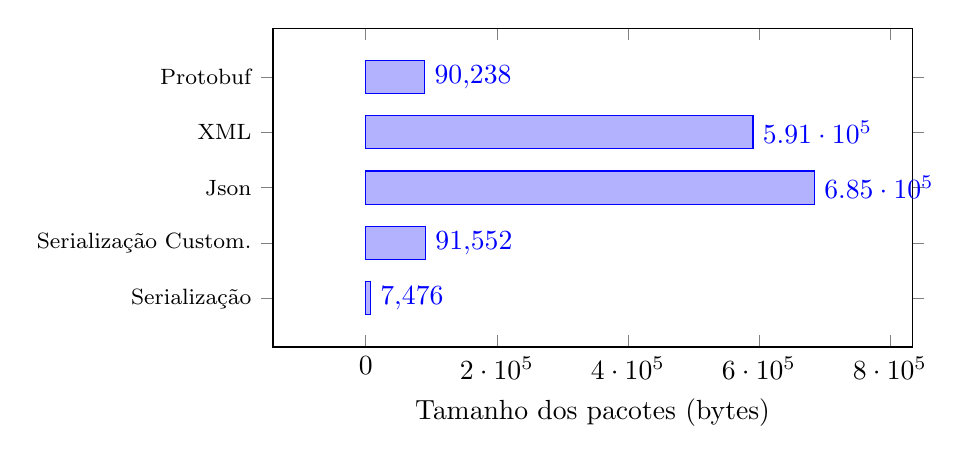
\begin{tikzpicture}
        \begin{axis}[
            symbolic y coords={ Serialização, Serialização Custom., Json, XML, Protobuf},
            xbar,
            scaled ticks = false,
            scaled x ticks = false,
            bar width=12pt,
            enlargelimits=0.22,
            y=20pt,
            width=0.8\textwidth,
            xlabel={Tamanho dos pacotes (bytes)},
            ytick=data,
            nodes near coords,
            nodes near coords align={horizontal},
            yticklabel style={font=\footnotesize, anchor=east}, % Gira os ticks em 45 graus
            ]
            \addplot coordinates {
                (7476,Serialização) 
                (91552,Serialização Custom.) 
                (684942,Json) 
                (590984,XML) 
                (90238,Protobuf)
                };
        \end{axis}
    \end{tikzpicture}
    \caption{Agenda de contatos}
\end{figure}
Para a agenda de contatos, colocação foi praticamente a mesma, o único detalhe foi que a Serialização ganhou disparado de todos os outros, isso se deve ao fato de termos usado a mesma foto em todos os contatos,ou seja, o mesmo ponteiro, então provalemente a Serialização percebeu isso enviu só uma vez.
De modo geral, o Protobuf é o mais eficiente em relação ao tamanho do pacote, mas é importante sempre analizar o problema e ver se existe uma forma melhor de transferir os seus dados para o seu caso, como a foi a Serialização que descobriu sozinha que a foto era a mesma em todos os contatos.

\appendix
\section{Json e XML}

\begin{lstlisting}[language=json, caption=Lista de compras Json.]
    {
        
        "lista_de_compras": [
            {
                "item": "Leite",
                "quantidade": 2,
                "unidade": "litros"
            },
            ...
            {
                "item": "Peito de Frango",
                "quantidade": 1,
                "unidade": "kg"
            }
        ]
    
    }
    \end{lstlisting}
    
    \begin{lstlisting}[language=xml, caption=Lista de compras XML.]
    <lista_de_compras>
        <item>
            <nome>Leite</nome>
            <quantidade>2</quantidade>
            <unidade>litros</unidade>
        </item>
        ...
        <item>
            <nome>Peito de Frango</nome>
            <quantidade>1</quantidade>
            <unidade>kg</unidade>
        </item>
    </lista_de_compras>
    \end{lstlisting}
    
    
    \begin{lstlisting}[language=json, caption=Agenda de contatos Json. Sem a foto e alguns contatos para não ficar muito grande.]
        {
            "contacts": [
                {
                    "name": "Alice Johnson",
                    "phone": "555-1234",
                    "email": "alice.johnson@example.com",
                    "photo": ...
                },
                ...
                {
                    "name": "Tina Yellow",
                    "phone": "555-5432",
                    "email": "tina.yellow@example.com",
                    "photo": ...
                }
            ]
        }
    \end{lstlisting}
    
    
    \begin{lstlisting}[language=xml, caption=Agenda de contatos XML. Sem a foto e alguns contatos para não ficar muito grande.]
    <contacts>
        <contact>
            <name>Alice Johnson</name>
            <phone>555-1234</phone>
            <email>alice.johnson@example.com</email>
            <photo>...</photo>
        </contact>
        ...
        <contact>
            <name>Tina Yellow</name>
            <phone>555-5432</phone>
            <email>tina.yellow@example.com</email>
            <photo>...</photo>
        </contact>
    </contacts>
    \end{lstlisting}
    
    
\end{document}